\documentclass[a4paper,11pt]{article}

\usepackage[lmargin=3cm,rmargin=3cm,tmargin=3cm,bmargin=3cm]{geometry}
\usepackage{amsmath}
\usepackage{amssymb}
\usepackage{graphicx}

\newcommand{\R}{\mathbb{R}}
\newcommand{\Z}{\mathbb{Z}}
\newcommand{\ceil}[1]{\left \lceil #1 \right \rceil}
\newcommand{\floor}[1]{\left \lfloor #1 \right \rfloor}
\begin{document}

\begin{center}
\bf
MATH1061/7861 | Discrete Mathematics

Selection from 2011 Semester 1 Exam | Week 11 Tutorial (T09)
\end{center}

These questions comprise about one-quarter of the available marks in the exam;
hence you should be able to complete these questions within approximately 30
minutes.

\begin{enumerate}
%\item {\bf 2010 Sem 2 Q1c}:
%%\begin{enumerate}
%%\item
%%Determine whether $p \land \sim q$ and $(p \lor q) \land \sim q$ are logically
%%equivalent.
%%\item
%%Is $(p \land q) \rightarrow (p \lor q)$ a tautology, contradiction,
%%or neither? Justify your answer.
%%\item
%Let $P(x,y)$ and $Q(x,y,z)$ be predicates defined
%for all real numbers $x, y, z$. Negate and simplify the following statement:
%\[
%    \forall x \in \R, \forall y \in \R \left[ P(x, y) \rightarrow
%    \left( \exists z \in \R \text{ such that } Q(x, y, z) \right) \right]
%\]
%\end{enumerate}

%\item {\bf 2012 Sem 1 Q4}:
%\begin{enumerate}
%\item
%Complete the following statement: ``if $a$ divides $b$ (that is, $a \mid b$) where
%$a$ and $b$ are integers, then $[\_\_\_] = [\_\_\_] \times k$ for some integer $k$''.
%\item
%If $a, b, c$ are integers such that $a \mid b$ and $b \mid c$, prove carefully
%that $a \mid (b + 2c)$.
%\item
%Prove that if $n$ is any odd integer, then $n^2-5$ is divisible by
%4 but never by 8.
%\end{enumerate}

%\item {\bf 2010 Sem 2 Q5}:
%Prove that $\sum_{k=1}^{n-1} k(k+1) = \frac{(n-1)n(n+1)}{3}$ for all $n \geq 2$.

% ~5 marks
\item[Q4.]
\begin{enumerate}
\item
Let $A = \{a, \emptyset\}$, $B = \{\emptyset\}$, $C = \{A, B, a\}$.

Complete the following (and remember curly braces where appropriate).
\begin{enumerate}
\item[(i)] $B-A = \dots$
\item[(ii)] $A \cup C = \dots$
\item[(iii)] $\mathcal{P}(A) = \dots$
\item[(iv)] $\mathcal{P}(A) \cap B = \dots$
\item[(v)] Is it true that $B \subseteq C$?
\end{enumerate}
\end{enumerate}

%\item {\bf 2012 Sem 1 Q6(b)(ii)}: A particular tree with 9 vertices has
%precisely five leaves, and precisely two vertices of degree 2.
%Find the degrees of the remaining two vertices.

% ~8 marks
\item[Q11.]
\begin{enumerate}
\item[(a)] For each of the following graphs $G$ and $H$,
write down either an Euler circuit or an Euler path, if either of these exist.
If neither exists, explain briefly why.

\begin{center}
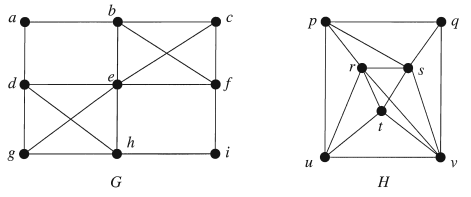
\includegraphics[scale=0.6]{src/1101q11a.png}
\end{center}

\item[(c)] A tree has 11 vertices. Exactly four of the vertices are leaves,
and six of the vertices have the same degree. Find the degree of all the
vertices. Show your working.\footnote{The original exam gave a different
wording for this question.}
\end{enumerate}

% 8 marks
\item[Q12.]
Let $f : \Z \to \Z$ and $g : \Z \to \Z$ be defined by
\[
    f(x) = \floor{\frac{x+1}{2}}, \quad g(x) = 2x + 1.
\]
Verify your answers below.
\begin{enumerate}
\item
What is the range of $f$?
\item
Is $f$ one-to-one?
\item
Is $f$ onto $\Z$?
\item
What is the range of $g$?
\item
Calculate $(g \circ f)(-4)$ and $(f \circ g)(-4)$.
\item
Calculate $(g \circ f)(x)$ and $(f \circ g)(x)$, and then show that if $x$ is
any {\em odd} integer then $(f \circ g)(x) = (g \circ f)(x) - 1$.
\end{enumerate}

% ~5 marks
\item[Q13.]
\begin{enumerate}
\item[(c)]
A binary relation $\alpha$ is defined on the
positive integers by: $x \, \alpha \, y$ if and only if $x+3y$ is even.
Is $\alpha$ reflexive? symmetric? transitive? Justify your answers.\footnote{The
original exam question only asked to simply state whether or not $\alpha$ was
reflexive, symmetric, and transitive. However, you should still know how to
justify your response.}

Is $\alpha$ an equivalence relation?
If so, give the equivalence classes; if not, explain why not.
\end{enumerate}

%\item {\bf 2012 Sem 1 Q11}:
%Let $f : \Z \to \Z$ be $f(x) = |2-x|$, $g(x) = \ceil{\frac{x}{2}}$.
%\begin{enumerate}
%\item
%What is the range of $f$?
%\item
%What is the range of $g$?
%\item
%Is $f$ one-to-one? Verify your answer.
%\item
%Is $g$ onto? Verify your answer.
%\item
%Find $(g \circ f)(3)$.
%\item
%Find $(f \circ g)(3)$.
%\item
%Is $g \circ f$ onto $\Z$? Verify your answer.
\end{enumerate}

\newpage

\begin{center}
\bf
MATH1061/7861 | Discrete Mathematics

Selection from 2011 Semester 1 Exam | Solutions | Week 11 Tutorial (T09)
\end{center}

\begin{enumerate}
\item[Q4.]
\begin{enumerate}
\item
%Let $A = \{a, \emptyset\}$, $B = \{\emptyset\}$, $C = \{A, B, a\}$.
\begin{enumerate}
\item[(i)] $B - A = \{\} = \emptyset$.
\item[(ii)] $A \cup C = \{a, \emptyset, A, B\}$.
\item[(iii)] $\mathcal{P}(A) = \{\emptyset, \{a\}, \{\emptyset\}, \{a, \emptyset\}\}$.
\item[(iv)] $\mathcal{P}(A) \cap B = \{\emptyset\}$.
\item[(v)] Is it true that $B \subseteq C$? {\em No}.
\end{enumerate}
\end{enumerate}

\item[Q11.]
\begin{enumerate}
\item[(a)]
An Euler path for $G$ is $c, b, a, d, e, b, f, c, e, f, i, h, d, g, e, h, g$.\footnote{Many
Euler paths exist, however they must start and finish at $c$ and $g$ (or vice versa).}

$H$ does not have an Euler circuit or an Euler path, since it has more than
two vertices of odd degree (namely $q, r, s, v$).

\item[(c)]
A tree on 11 leaves has 10 edges, hence total degree 20 (by the Handshake
Theorem). Precisely four vertices have degree 1, six share the same degree,
call it $a$, then there is one more vertex, let the degree of that vertex be
$b$. Then, $a, b \geq 2$, and
\[
    20 = 4 \cdot 1 + 6a + b \implies 16 = 6a + b.
\]
In particular, $6a < 16$, so $a < \frac{16}{6} < 3$, and since $a \geq 2$, we have $a = 2$.
Hence $b = 16 - 6a = 4$. Thus there are four vertices of degree 1,
six of degree 2, and one of degree 4.
\end{enumerate}

\item[Q12.]
%Let $f : \Z \to \Z$ and $g : \Z \to \Z$ be defined by
%\[
%    f(x) = \floor{\frac{x+1}{2}}, \quad g(x) = 2x + 1.
%\]
\begin{enumerate}
\item The range of $f$ is $\Z$: for any $y \in \Z$, we have
$f(2y) = \floor{y+\frac{1}{2}} = y$, so every $y \in \Z$ is the image of
some $x \in \Z$ (where $x=2y$).
\item $f$ is not one-to-one: for example, $f(1) = \floor{1} = 1$ and
$f(2) = \floor{\frac{3}{2}} = 1 = f(1)$.
\item $f$ is onto, since the range is equal to the codomain (by part (a) above).
\item The range of $g$ is the set of all odd numbers (by definition of an odd
number).
\item $(g \circ f)(-4) = g\left( \floor{\frac{-3}{2}} \right) = g(-2) = -3$,
\quad
$(f \circ g)(-4) = f(-7) = \floor{-3} = -3$.
\item
$(g \circ f)(x) = 2 \floor{\frac{x+1}{2}} + 1$, and
$(f \circ g)(x) = \floor{\frac{(2x+1)+1}{2}} = \floor{x+1} = x+1$.
Now, suppose $x$ is odd. To show that $(f \circ g)(x) = (g \circ f)(x)-1$, we
need to show that $(g \circ f)(x) = x+2$.

If $x$ is odd, then $x = 2k+1$ for some $k \in \Z$, therefore
\[ (g \circ f)(x) = 2 \floor{\frac{2k+2}{2}} + 1 = 2 (k+1) + 1 = 2k+3 = x+2. \]

{\em Alternatively:} if $x$ is odd, then $x = g(k)$ for some $k \in \Z$,
so
\[ (g \circ f)(x) = ((g \circ f) \circ g)(k) = (g \circ (f \circ g))(k) = g(k+1) = 2k+3 = x+2. \]
\end{enumerate}

\item[Q13.]
\begin{enumerate}
\item[(c)]
\begin{itemize}
\item
$\alpha$ is reflexive: for all $x \in \Z$, $x+3x = 4x$ is even, so $x \,\alpha\, x$.
\item
$\alpha$ is symmetric: for all $x, y \in \Z$, if $x \, \alpha \, y$, then
$x+3y$ is even, hence $y+3x = (x+3y) + 2(x-y)$ is the sum of two even numbers,
so is even.
\item
$\alpha$ is transitive: for all $x, y, z \in \Z$, if $x \, \alpha \, y$ and
$y \,\alpha\, z$, then $x+3y$, $y+3z$ are even, and so
$x+3z = (x+3y) + (y+3z) - 4y$ is the sum of even numbers, hence is even, so
$x \,\alpha\, z$.
\end{itemize}
Therefore, $\alpha$ is an equivalence relation. Note that $x \,\alpha\, y$ iff
$x$ and $y$ have the same parity (i.e. both even or both odd), hence the
equivalence classes are $[0] = \{\dots, -2, 0, 2, 4, \dots\}$ and
$[1] = \{\dots, -3, -1, 1, 3, \dots\}$.
\end{enumerate}
\end{enumerate}

\end{document}
